\subsection{Inteligencia Artificial}
La Inteligencia Artificial es la inteligencia llevado a cabo por máquinas en las que una máquina “inteligente” ideal es un agente flexible que percibe su entorno y lleva a cabo acciones que maximicen sus posibilidades de éxito en algún objetivo \parencite{tec_poole1998machinelearning}. Este término se aplica cuando una máquina imita las funciones “cognitivas” que asocian los humanos con otras mentes \parencite{bk_russell2009intart}.

Durante la historia de la humanidad, se han seguido 4 enfoques: dos centrados en el comportamiento humano y dos enfocados en torno a la racionalidad. El enfoque centrado en el comportamiento humano se basa en una ciencia empírica, es decir, mediante experimentos que incluyen hipótesis y confirmaciones. Este enfoque nace a partir de la prueba de Alan Turing, en 1950, en la cual, el célebre matemático inglés diseñó una prueba basada en la incapacidad de diferenciar entre entidades inteligentes indiscutibles y seres humanos por parte de un computador. Si este era capaz de diferenciar y superar la prueba mientras que el humano no, se afirma que se trataba de una “máquina inteligente”. Por ello, el computador debía contar con las siguientes capacidades: procesamiento de lenguaje natural para poder comunicarse, representación del conocimiento describiendo lo que percibe de su entorno, razonamiento automático utilizando la información procesada en su interior, y aprendizaje automático para adaptarse a nuevos eventos. Si el evaluador decide incluir una señal de video para evaluar la percepción de la computadora, se dice que se está realizando la Prueba Global de Turing. Para superarla, además de las 4 anteriormente mencionadas, la computadora debe contar además con las capacidades de visión computacional para percibir objetos y robótica con el fin de manipularlos. Todas estas seis capacidades o disciplinas abarcan la mayor parte de la Inteligencia Artificial \parencite{bk_russell2004intart}.

Por el otro lado, el enfoque racional implica una combinación de ingeniería y matemáticas basándose en las “leyes del pensamiento”. Estas parten de la Grecia antigua, planteadas por grandes filósofos como Aristóteles en su intento de codificar la “manera correcta de pensar”, lo que más adelante derivó al estudio de la lógica. Más adelante, en el siglo XIX, se construyeron programas capaces de resolver problemas en notación lógica. De ahí que la tradición logista dentro del campo de la Inteligencia Artificial trata de construir sistemas inteligentes con estas capacidades. De todo lo anterior dicho respecto al enfoque racional se creó el término de un agente racional, el cual actúa intentando lograr el mejor resultado, o de existir incertidumbre, el mejor resultado esperado. Finalmente, la amplia aplicación de la Inteligencia Artificial y sus fundamentos derivan en muchas ciencias de las cuales se pueden mencionar, además de la filosofía y las matemáticas, a la economía, neurociencia, psicología, la ingeniería computacional, la teoría de control y cibernética, y hasta la lingüística \parencite{bk_russell2004intart}.

Pero, ¿cómo es surge este amplio estudio de la Inteligencia Artificial? En 1943, basándose en la fisiología básica y funcionamiento de las neuronas en el cerebro, el análisis formal de la lógica proposicional de Russell y Whitehead, y la teoría computacional de Turing, dos estudiosos en neurociencia realizaron juntos el que sería considerado primer trabajo de Inteligencia Artificial. Warren McCulloch y Walter Pitts propusieron un modelo constituido por neuronas artificiales, en el que cada una de ellas se caracterizaba por estar “activada” o “desactivada”; la del primer tipo daba como resultado a la estimulación producida por una cantidad suficiente de neuronas vecinas. Como ejemplo, mostraron que cualquier función de cómputo podría calcularse mediante alguna red de neuronas interconectadas y que todos los conectores lógicos eran capaces de ser implementados usando estructuras sencillas de red. Seis años más adelante, Donald Hebb propuso una regla de actualización de intensidades de conexiones entre las neuronas, la que actualmente se le conoce como la “regla de aprendizaje Hebbiano” vigente hasta nuestros días. En 1956, Allen Newell y Herbert Simon inventaron un programa de computación en el taller de Dartmouth de John McCarthy, que era capaz de pensar de forma no numérica, basado en el Teórico Lógico, artículo que, además, fue rechazado de ser publicado en la revista \textit{Journal of Symbolic Logic}. A pesar de ello, los trabajos de los colaboradores presentes en dicho taller se mantuvieron por 20 años más, siendo McCarthy quien acuñó el término de “Inteligencia Artificial” a este campo \parencite{bk_russell2004intart}.

En la década de los años 80, la Inteligencia Artificial dio el gran salto de formar parte de la industria, en especial, de las compañías más grandes de los países desarrollados a través de grupos especializados para la realización de investigaciones de sistemas expertos, así como en la construcción de computadoras cada vez más potentes y capaces de resolver tareas más complejas.

Actualmente, la IA cuenta con muchas aplicaciones como la Minería de Datos, el procesamiento de lenguaje natural, la robótica, los videojuegos, entre otros. Dentro de ella se pueden encontrar otras ramas como por ejemplo el Aprendizaje Automático, Visión computacional, etcétera.

\subsection{Aprendizaje Automático}
El Aprendizaje Automático (\textit{Machine Learning} por su nombre en inglés) es una rama de la Inteligencia Artificial cuyo fin es desarrollar técnicas que las computadoras pueden aprender a través de encontrar algoritmos y heurísticas que conviertan muestras de datos en programas sin necesidad de hacerlos \parencite{bk_russell2009intart}. Sus algoritmos están compuestos por muchas tecnologías, como por ejemplo Aprendizaje Profundo, Redes Neuronales y Procesamiento de lenguaje natural, utilizadas en el aprendizaje supervisado y no supervisado, las cuales operan guiadas por lecciones de información existente \parencite{gl_gartner2019ml}. La premisa básica del aprendizaje automático es construir algoritmos que puedan recibir datos de entrada y usar análisis estadísticos para predecir una salida mientras se actualizan las salidas a medida que se dispone de nuevos datos \parencite{bk_alpaydin2014ml}.

Los tres tipos de aprendizaje principales son:
\begin{itemize}
	\item \textbf{Aprendizaje supervisado}: Se trabajan con datos etiquetados buscando obtener una función que asigne una respuesta de salida adecuada, denominadas etiquetas, a partir de unos datos de entrada denominadas características \parencite{bk_zambrano2018supnosup}. Por lo general, los datos de entrada son conocidos como variables dependientes o X, mientras que los datos de salida son llamadas variables independientes o Y. Se le dice supervisado ya que el resultado depende de los datos que recibe de entrada, afectando su performance si estos son alterados.
	
	Existen dos tipos de aprendizaje supervisado. El primero es la regresión, que consiste en obtener como resultado un número específico a partir de un conjunto de variables de las características, representado en la Figura \ref{2:fig1}; mientras que por otra parte está la clasificación, el cual se basa en encontrar distintos patrones ocultos para clasificar los elementos del conjunto de datos en diferentes grupos, como se aprecia en la Figura \ref{2:fig2} \parencite{bk_zambrano2018supnosup}.
	\begin{figure}[htbp]
		\begin{center}
			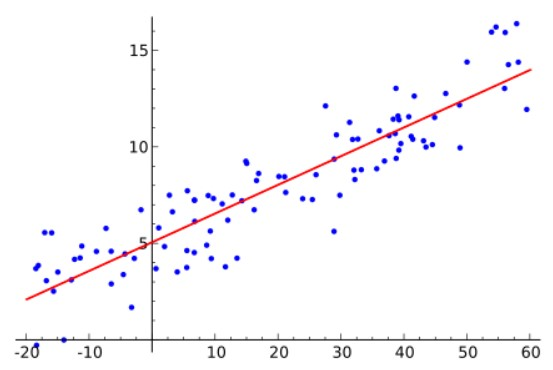
\includegraphics[width=0.6\textwidth]{2/figures/regresion.jpg}
			\caption{Ejemplo de algoritmo de regresión. Fuente: \cite{bk_zambrano2018supnosup}}
			\label{2:fig1}

			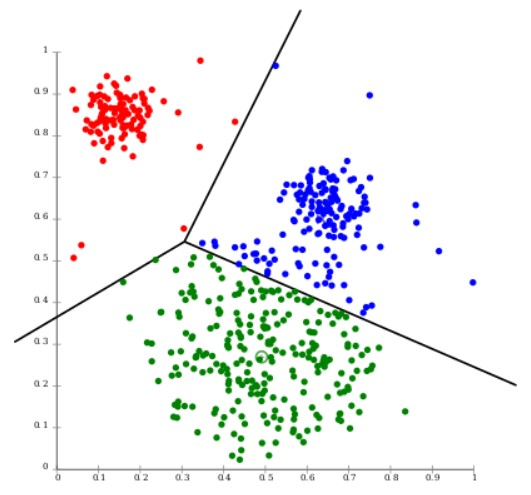
\includegraphics[width=0.5\textwidth]{2/figures/clasificacion.jpg}
			\caption{Ejemplo de algoritmo de clasificación. Fuente: \cite{bk_zambrano2018supnosup}}
			\label{2:fig2}
		\end{center}
	\end{figure}
	
	Para el segundo tipo de aprendizaje supervisado, el algoritmo más usado es el de los K Vecinos más cercanos o \textit{k-NN Nearest Neighbour} en inglés. Este se basa en la idea de que los nuevos ejemplos serán clasificados a la clase a la cual pertenezca la mayor cantidad de vecinos más cercanos del conjunto de entrenamiento más cercano a él. Sin embargo, el número k de vecinos más cercanos lo decide el usuario, de preferencia impar, para evitar ambigüedad al momento de clasificar un registro por parte del algoritmo (esto puede ocasionarse por las mismas distancias existentes entre dos o más registros). Otra variante aplicada consiste en la ponderación de cada vecino de acuerdo a la distancia entre él y el ejemplar a ser clasificado, asignando mayor peso a los más próximos \parencite{tec_sancho2018supnosup}. Por ejemplo, si x es el ejemplo que se desea clasificar, V son las posibles clases de clasificación, yxi es el conjunto de los k ejemplos de entrenamiento más cercano, se define la siguiente fórmula:
	
	y finalmente, la clase asignada a x es aquella que verifique que la suma de los pesos de sus representantes sea la máxima, representándose en la Figura \ref{2:fig3}:
	\begin{figure}[h]
		\begin{center}
			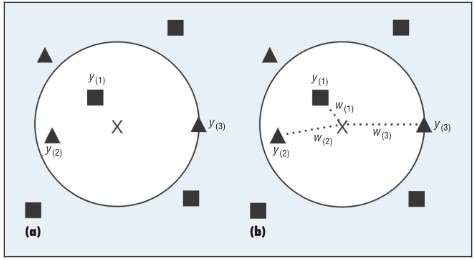
\includegraphics[width=0.6\textwidth]{2/figures/knn.jpg}
			\caption{Algoritmo de K Vecinos más cercanos con pesos ponderados. Fuente: \cite{tec_sancho2018supnosup}}
			\label{2:fig3}
		\end{center}
	\end{figure}
	
	\item \textbf{Aprendizaje no supervisado}: A diferencia de la anterior, aquí se trabaja con datos no etiquetados para entrenar el modelo, ya que el fin es de carácter exploratorio y descriptivo de la estructura de los datos. No existen variables independientes o Y.
	
	La función es agrupar ejemplares, por lo que el algoritmo los cataloga por similitud en sus características y a partir de ahí, crea grupos o clústeres sin tener la capacidad de definir cómo es cada individualidad de cada uno de los integrantes de los mismos \parencite{bk_zambrano2018supnosup}.
	
	El algoritmo usado para este tipo de aprendizaje es el de las K medias o \textit{k-means} en inglés. Este intenta encontrar una partición de las muestras en K agrupaciones, de manera que cada ejemplar pertenezca a una de ellas de acuerdo al centroide más cercano. Si bien el valor de K es definido por el usuario, a partir de pruebas de varias iteraciones se le puede consultar al algoritmo cuál es su valor óptimo. La intención es minimizar la varianza total del sistema. Por ejemplo, si se tiene el centroide ci de la agrupación i-ésima, yxji es el conjunto de ejemplos clasificados en esa agrupación, la función para lograr esto es la siguiente:
	
	Representándose en la Figura \ref{2:fig4}, los pasos seguidos para este algoritmo comienzan con la selección de los K puntos como como centros de los grupos. Luego, se asignarán los ejemplos al centro más cercano y se calculará el centroide de los ejemplos asociados a cada grupo. Finalmente, estos dos últimos pasos se repetirán hasta que ninguno de los centros pueda ser reasignados en las iteraciones.
	\begin{figure}[h]
		\begin{center}
			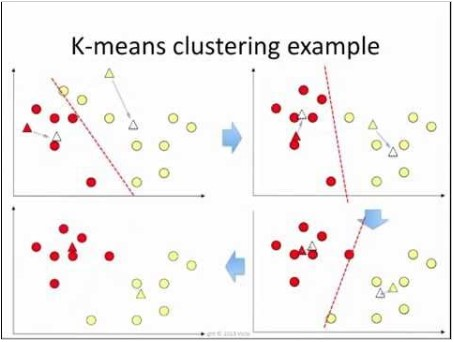
\includegraphics[width=0.6\textwidth]{2/figures/kmeans.jpg}
			\caption{Funcionamiento del algoritmo de K medias. Fuente: \cite{tec_sancho2018supnosup}}
			\label{2:fig4}
		\end{center}
	\end{figure}
		
	\item \textbf{Aprendizaje por refuerzo}: Se basa en que un agente racional puede tomar una decisión a partir de una retroalimentación llamada recompensa o refuerzo. A diferencia del Aprendizaje Supervisado, en donde el agente puede aprender solamente a partir de ejemplos dados, en este caso no basta solamente con proporcionárselos sino también de “informarle” si lo está haciendo de la manera correcta o no. Por ejemplo, un agente que intenta aprender a jugar ajedrez necesita saber que algo bueno ha ocurrido cuando gana y algo malo ha ocurrido cuando pierde. La mejor recompensa que busca al finalizar el juego es vencer al oponente, y para ello debe estudiar todos los movimientos que este haga, la posición de las fichas en el tablero, entre otros. A este conjunto se le conoce como entorno o medio ambiente \parencite{bk_russell2004intart}. Entonces, en resumen, representando en la Figura \ref{2:fig5}, y mencionando otro ejemplo, el aprendizaje por refuerzo está compuesto por un agente (Pacman) en un estado determinado (su ubicación o posición actual) dentro de un medio ambiente (el laberinto). La recompensa positiva que busca Pacman son los puntos por comer, mientras que la negativa será la de morir si se cruza con un fantasma, en base a la acción (desplazamiento a un nuevo estado) que realice \parencite{tec_merino2019aprendrefuerzo}.
	\begin{figure}[h]
		\begin{center}
			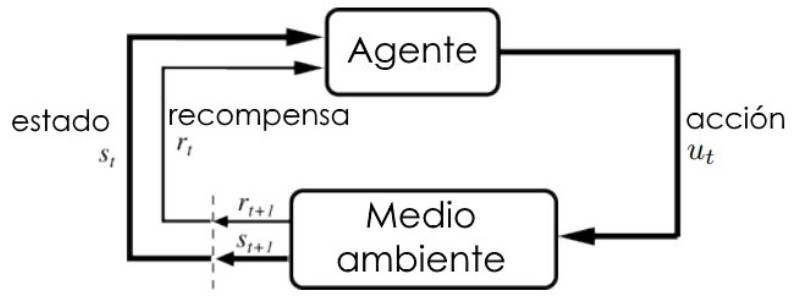
\includegraphics[width=0.7\textwidth]{2/figures/aprendizaje_refuerzo.jpg}
			\caption{Componentes del Aprendizaje por Refuerzo. Fuente: \cite{bk_sutton2018rl}}
			\label{2:fig5}
		\end{center}
	\end{figure}
\end{itemize}

\subsection{Aprendizaje Profundo}
El Aprendizaje Profundo (\textit{Deep Learning} por su nombre en inglés) es un tipo de Aprendizaje Automático que entrena a una computadora para que realice tareas como las realizadas por los seres humanos, desde la identificación de imágenes hasta realizar predicciones y reconocer el lenguaje humano. El Aprendizaje Profundo configura parámetros básicos acerca de los datos y entrena a la computadora para que aprenda por su cuenta reconociendo patrones mediante el uso de múltiples capas de procesamiento \parencite{gl_sas_deeplearning}. Se basa en teorías acerca de cómo funciona el cerebro humano \parencite{tec_banafa2019deeplearning}.

La principal diferencia con el Aprendizaje Automático es que el Aprendizaje Profundo se basa en la extracción de características y clasificación al mismo tiempo luego de recibir una entrada, algo que en la primera técnica ocurre por separado, como se aprecia en la Figura \ref{2:fig6}.
\begin{figure}[h]
	\begin{center}
		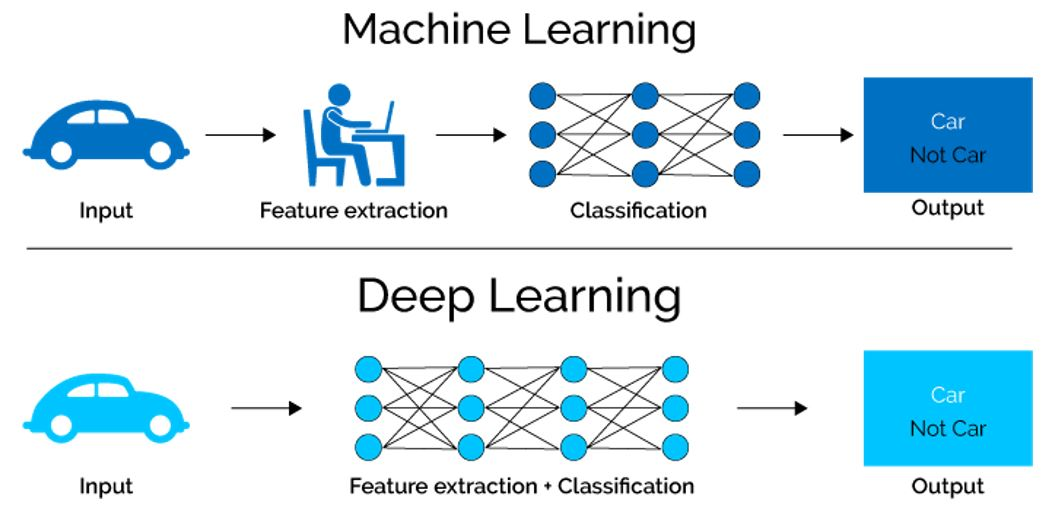
\includegraphics[width=0.8\textwidth]{2/figures/deeplearning_machinelearning.jpg}
		\caption{Diferencia entre Aprendizaje Automático y Aprendizaje Profundo. Fuente: \cite{tec_cook2018deeplearning}}
		\label{2:fig6}
	\end{center}
\end{figure}

Por un lado, mientras en el aprendizaje automático o de máquina, el ordenador extrae conocimiento a través de experiencia supervisada, en el aprendizaje profundo está menos sometido a supervisión. Mientras que el primer tipo de aprendizaje consume muchísimo tiempo y se basa en proponer abstracciones que permiten aprender al ordenador, en el segundo no consume demasiado tiempo y por el contrario de su par, crea redes neuronales a gran escala que permiten que el ordenador aprenda y piense por sí mismo sin necesidad directa de intervención humana. Actualmente, el aprendizaje profundo se usa para crear softwares capaces de determinar emociones o eventos descritos en textos, reconocimiento de objetos en fotografías y realizar predicciones acerca del posible comportamiento futuro de las personas. Empresas como Google (proyecto Google Brain) o Facebook (Unidad de investigación en IA) han puesto en marcha proyectos basados en esta rama para potenciar y mejorar sus algoritmos con el fin de ofrecer una mejor experiencia de sus servicios a sus clientes \parencite{tec_banafa2019deeplearning}.

\subsection{Modelo Predictivo}
Son modelos de datos estadísticos utilizados para predecir el comportamiento futuro. En estos, se recopilan datos históricos y actuales, se formula un modelo estadístico, se realizan predicciones y el modelo se valida a medida que se dispone de datos adicionales. Los modelos predictivos analizan el rendimiento pasado para evaluar la probabilidad de que un cliente muestre un comportamiento específico en el futuro. En esta categoría también abarca la búsqueda de patrones ocultos \parencite{gl_gartner2019pm}.

\subsection{Minería de Datos}
La Minería de Datos es un campo de la estadística y las ciencias de la computación referido al proceso que intenta descubrir patrones en grandes volúmenes de conjuntos de datos \parencite{bk_maimon2010datamining}. Normalmente, estos patrones no pueden detectarse mediante la exploración tradicional de datos porque sus relaciones son demasiado complejas o por su gran volumen. Para ello, utiliza métodos de Inteligencia Artificial, Aprendizaje Automático, estadística y sistemas de bases de datos. Estos patrones son recopilados y definidos como un modelo de minería de datos, los cuales pueden aplicarse en los siguientes escenarios \parencite{gl_microsoft2019datamining}:
\begin{itemize}
	\item Previsión.
	\item Riesgo y probabilidad.
	\item Recomendaciones.
	\item Buscar secuencias.
	\item Agrupación.
\end{itemize}

La generación de un modelo de minería de datos forma de un macro-proceso descrita en los siguientes seis pasos representados en la Figura \ref{2:fig7} \parencite{gl_microsoft2019datamining}:
\begin{figure}[h]
	\begin{center}
		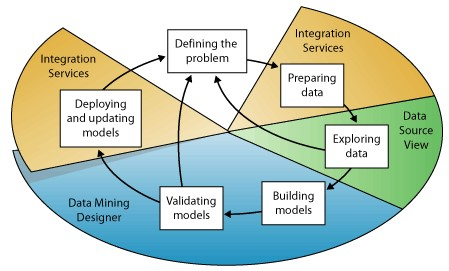
\includegraphics[width=0.7\textwidth]{2/figures/data_mining_steps.jpg}
		\caption{Diagrama de los seis pasos básicos. Fuente: \cite{gl_microsoft2019datamining}}
		\label{2:fig7}
	\end{center}
\end{figure}

\subsection{Metodologías de Minería de Datos}
Dentro de los sistemas de analítica de negocio, Big Data y Minería de Datos, las tres metodologías más usadas se encuentran CRISP-DM, SEMMA y KDD \parencite{tec_braulio2015metodologiasdm}.
\begin{itemize}
	\item \textbf{CRISP-DM} (Cross Industry Standard Process for Data Mining):
	
	Esta metodología presenta seis fases representadas en la Figura \ref{2:fig8} a continuación.
	\begin{figure}[h]
		\begin{center}
			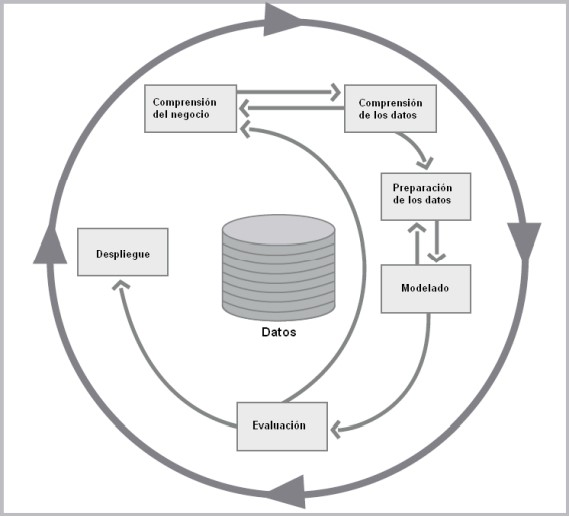
\includegraphics[width=0.75\textwidth]{2/figures/crispdm.jpg}
			\caption{Fases de la metodología CRISP-DM. Fuente: \cite{tec_braulio2015metodologiasdm}}
			\label{2:fig8}
		\end{center}
	\end{figure}
		
	\begin{itemize}
		\item En la comprensión del negocio se determinan los objetivos y requerimientos desde el lado del negocio, así como generar plan del proyecto.
		\item En la comprensión de los datos se logra entender el significado de las variables existentes, así como el entendimiento de los datos desde su recopilación hasta su verificación de calidad.
		\item En la preparación de los datos se prepara el conjunto de datos adecuado que servirán para la construcción del modelo. Por ello, la calidad de los datos es un factor relevante y ello requiere la exclusión de redundancia y valores que no ayuden a establecer buena comprensión y resultados más adelante. A esto se le conoce como limpieza de datos.
		\item En el modelado se aplican técnicas de minería de datos en el conjunto de datos creado en el paso anterior. Para ello, se evalúan entre varias la que mejor performance desempeñe y luego se construye el o los modelos que busquen determinar un objetivo.
		\item En la evaluación se evalúan los posibles modelos del paso anterior a partir del nivel de importancia de acuerdo a las necesidades del negocio y performance que estos cuentan.
		\item El despliegue, finalmente, utiliza el modelo final creado para determinar los objetivos que se buscan cumplir en los requerimientos y ayudar en la toma de decisiones.
	\end{itemize}
	
	\item \textbf{SEMMA} (Sample – Explore – Modify – Model – Assess):
	
	Esta metodología cuenta con cinco fases como se aprecia en la Figura \ref{2:fig9}. A diferencia de la anterior, esta metodología se enfoca más en el modelado.
	\begin{figure}[h]
		\begin{center}
			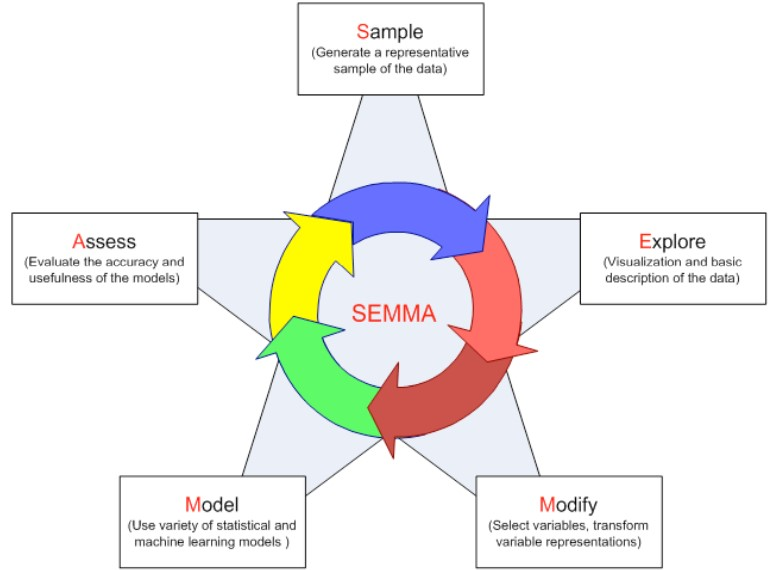
\includegraphics[width=0.75\textwidth]{2/figures/semma.jpg}
			\caption{Fases de la metodología SEMMA. Fuente: \cite{tec_braulio2015metodologiasdm}}
			\label{2:fig9}
		\end{center}
	\end{figure}
	
	\begin{itemize}
		\item En la Muestra (Sample) se crea una muestra significativa.
		\item En la Exploración (Explore) se comprenden los datos con el fin de encontrar relaciones entre variables y anomalías.
		\item En la Modificación (Modify) se transforman las variables para las necesidades del modelo.
		\item En la Modelización (Model) se aplican uno o varios modelos sobre el conjunto de datos para buscar resultados.
		\item En el Asesoramiento (Assessment) se evalúan los resultados obtenidos del modelo.
	\end{itemize}
	
	\item \textbf{KDD} (Knowledge Discovery and Data Mining):
	
	Esta metodología se refiere al proceso de encontrar conocimiento alguno en el dato y, a diferencia de sus predecesores, se enfoca en crear aplicaciones de minería de datos. Consta de cinco fases más 1 previa y 1 posterior basadas en la generación de conocimiento como se muestra en la Figura \ref{2:fig10}.
	\begin{figure}[h]
		\begin{center}
			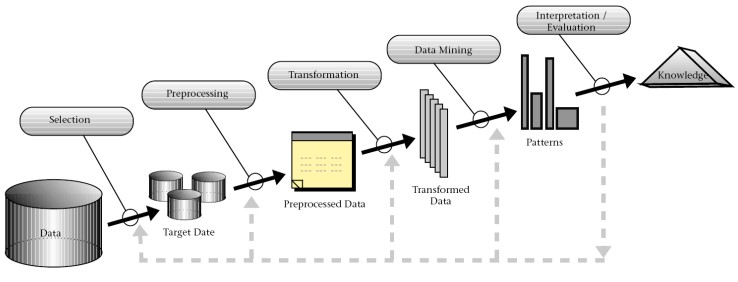
\includegraphics[width=0.75\textwidth]{2/figures/kdd.jpg}
			\caption{Fases de la metodología KDD. Fuente: \cite{tec_braulio2015metodologiasdm}}
			\label{2:fig10}
		\end{center}
	\end{figure}
	
	\begin{itemize}
		\item En la fase Pre KDD se comprende el dominio del negocio, así como también se identifican las necesidades del cliente.
		\item En la selección, primero se identifica el conjunto de datos a usar y luego se seleccionan la muestra y las variables para la exploración.
		\item En el pre-procesamiento, se realiza la limpieza de datos y se elimina el ruido, así como los valores atípicos.
		\item En la transformación se implementan métodos de reducción de dimensiones para reducir el número de variables efectivas.
		\item En la Minería de datos, se elige el tipo de tarea de minería de datos (clasificación, regresión, agrupamiento, entre otros) así como el algoritmo, los métodos, los modelos y parámetros apropiados.
		\item En la interpretación y evaluación se analizan los resultados dados.
		\item En la fase Post KDD finalmente se consolida el conocimiento adquirido.
	\end{itemize}

\end{itemize}

Luego de presentar las tres metodologías más usadas, la pregunta dada es ¿cuál de los tres representa la mejor opción para usar?
Las tres metodologías tienen distinto número de pasos, así como distintos enfoques, tal cual se observa en el siguiente resumen de la Tabla \ref{2:table1}.

\begin{table}[htbp]
	\newcommand{\multirot}[1]{\multirow{2}{*}[-8ex]{\rotcell{\rlap{#1}}}}
	%\scriptsize
	\footnotesize
	\centering
	\begin{tabular}{|M{3cm}|M{5cm}|M{3.5cm}|M{3.5cm}|}
		\hline
		\rowcolor[rgb]{0,0.251,0.502}
		\multicolumn{1}{|p{3cm}|}{\centering \textcolor{white}{Modelo de Procesos de Minería de Datos}} &
		\multicolumn{1}{|p{5cm}|}{\centering \textcolor{white}{KDD}} &
		\multicolumn{1}{|p{3.5cm}|}{\centering \textcolor{white}{CRISP-DM}} & 
		\multicolumn{1}{|p{3.5cm}|}{\centering \textcolor{white}{SEMMA}}
		\\
		\hline
		{Número de pasos}
		&9
		&6
		&5                                                        
		\\
		\hline
		{\multirow{9}{*}[-11ex]{Nombre de los pasos}}
		&Desarrollo y entendimiento de la aplicación
		&Entendimiento del negocio
		&- \\
		\cline{2-4}
		&Creación de un conjunto de datos de destino
		&\multirow{2}{*}[-2ex]{Entendimiento de los datos}
		&Muestreo
		\\
		\cline{2-2}\cline{4-4}
		&Limpieza de datos y pre-procesamiento
		&\multicolumn{1}{c|}{}
		&Exploración
		\\
		\cline{2-4}
		&Transformación de datos
		&Preparación de los datos
		&Modificación
		\\
		\cline{2-4}
		&Elección de la tarea adecuada de Minería de datos
		&\multirow{3}{*}[-3ex]{Modelamiento}
		&\multirow{3}{*}[-3ex]{Modelo}
		\\
		\cline{2-2}
		&Elección del algoritmo adecuado de Minería de datos
		&\multicolumn{1}{c|}{}
		&\multicolumn{1}{c|}{}
		\\
		\cline{2-2}
		&Implementación del algoritmo de Minería de datos
		&\multicolumn{1}{c|}{}
		&\multicolumn{1}{c|}{}
		\\
		\cline{2-4}
		&Interpretación de patrones minados
		&Evaluación
		&Evaluación
		\\
		\cline{2-4}          & Uso de conocimiento descubierto & Despliegue & -
		\\
		\hline
	\end{tabular}%
	\caption{Cuadro comparativo entre características de las tres metodologías. Fuente: \cite{tec_shafique2014dmmodels}}
	\label{2:table1}
\end{table}

Sin embargo, la elección depende de los involucrados que finalmente usarán el modelo en el negocio. La mayoría de investigadores siguen la metodología KDD debido a que es más completo y su exactitud. Para aquellos objetivos enfocados más en la compañía como la integración usada por SAS Enterprise Miner con su software se utilizan SEMMA y CRISP-DM. Esta última resulta ser más completa de acuerdo a los estudios.

\subsection{Técnicas de Minería de Datos}
Existe una gran variedad de técnicas para la Minería de Datos. Las más importantes y utilizadas en los antecedentes de la investigación se mencionan a continuación \parencite{gl_microsoft2018datamining}.

\begin{itemize}
	\item \textbf{Redes Neuronales Artificiales} (RNA): Es un sistema de computación que consiste en un número de elementos o nodos simples, pero altamente interconectados, llamados “neuronas”, que se organizan en capas que procesan información utilizando respuestas de estado dinámico a entradas externas \parencite{tec_inzaugarat2018ann}.
	
	Este sistema de programas y estructura de datos se aproxima al funcionamiento del cerebro humano. Una red neuronal implica tener un gran número de procesadores funcionando en paralelo, teniendo cada uno de ellos su propia esfera de conocimiento y acceso a datos en su memoria local. Normalmente, una se alimenta con grandes cantidades de datos y un conjunto dado de reglas acerca de las relaciones. Luego, un programa puede indicar a la red cómo debe comportarse en respuesta a un estímulo externo o si puede iniciar la actividad por sí misma \parencite{tec_banafa2019deeplearning}.
	
	Para entender mejor cómo funciona una red neuronal, hay que describir qué es una neurona. Una neurona es una célula del cerebro cuya función principal es la recogida, procesamiento y emisión de señales eléctricas. Debido a que se piensa que la capacidad de procesamiento de información del cerebro proviene de redes de este tipo de neuronas, los primeros trabajos en Inteligencia Artificial se basaron en crear redes neuronales artificiales para emular este comportamiento, en 1943 con un modelo matemático, mostrado en la Figura \ref{2:fig11}, por los ya mencionados anteriormente McCulloch y Pitts. Estos y posteriores trabajos potenciaron lo que hoy en día se conoce como el campo de la neurociencia computacional \parencite{bk_russell2004intart}. Años más tarde, en 1958, se desarrolló el concepto del perceptrón por Rosenblatt, el cual tenía la capacidad de aprender y reconocer patrones sencillos, formado por entradas, neurona, función de adaptación (sigmoidal, tangencial, en escalón, etc.) y salida.
	\begin{figure}[h]
		\begin{center}
			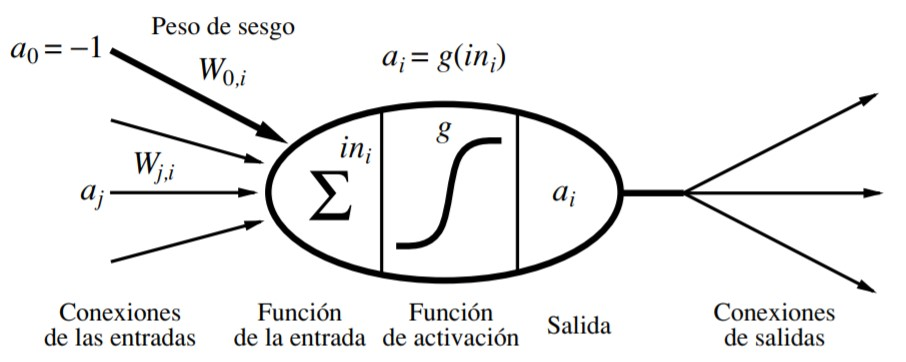
\includegraphics[width=0.75\textwidth]{2/figures/rnn_mcculloch.jpg}
			\caption{Modelo para representar una neurona propuesto por McCulloch y Pitts (1943). Fuente: \cite{bk_russell2004intart}}
			\label{2:fig11}
		\end{center}
	\end{figure}
	
	La última figura descrita muestra, además de los pesos, funciones de activación tanto para la entrada (aj) como para la salida (ai). Pero, ¿qué son estas funciones y para qué sirven?
	
	Para comenzar, las redes neuronales están compuestas de nodos (la elipse) conectados a través de conexiones dirigidas (las flechas). Una conexión del nodo j a la unidad i sirve para propagar la activación aj de j a i. Asimismo, cada conexión tiene un peso numérico W(j,i) que determina la fuerza y el signo de la conexión. Para calcular cada nodo i, se realiza una suma ponderada de sus entradas (producto entre pesos y nodos de entrada j), y se le añade el sesgo (bias) teta-i (aumenta/disminuye el valor de la combinación lineal de las entradas):
	
	Posteriormente, se efectúa una función de activación g a esta suma para producir la salida:
	
	Entonces, aquí se explica los dos objetivos de una función de activación. En primer lugar, se desea que el nodo esté “activo” (cercano a +1) cuando las entradas correctas sean dadas, e “inactiva” (cercano a 0) cuando las entradas erróneas sean proporcionadas. En segundo lugar, la activación tiene que ser no lineal porque, de lo contrario, la red neuronal colapsaría en su totalidad con una función lineal sencilla, como se aprecia en el ejemplo de la Figura \ref{2:fig12}.
	\begin{figure}[h]
		\begin{center}
			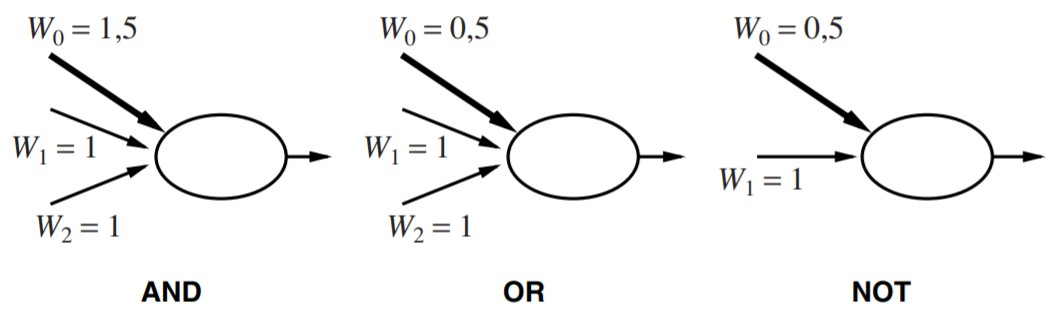
\includegraphics[width=0.75\textwidth]{2/figures/rna_activaciones.jpg}
			\caption{Nodos con funciones de activación umbral en forma de puertas lógicas. Fuente: \cite{bk_russell2004intart}}
			\label{2:fig12}
		\end{center}
	\end{figure}
	
	Entre las funciones de activación que más destacan son las siguientes:
	\begin{itemize}
		\item \textbf{Función sigmoide o logística}: Toma los valores de entrada que oscilan entre infinito negativo y positivo, y restringe los valores de salida al rango entre 0 y 1. Frecuentemente es usada en Redes Multicapa (MLP) entrenadas con el algoritmo de propagación inversa. Se representa como en la Figura \ref{2:fig13} y su fórmula para calcular su nuevo valor es:
		\begin{figure}[h]
			\begin{center}
				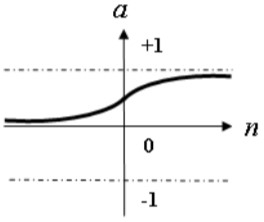
\includegraphics[width=0.3\textwidth]{2/figures/sigmoide.jpg}
				\caption{Función de activación sigmoide. Fuente: \cite{pr_dorofki2012ann}}
				\label{2:fig13}
			\end{center}
		\end{figure}
		
		Un dato curioso de esta función relacionado con la regresión logística es que el nombre de esta última no deriva de una regresión. Por el contrario, se debe a que, al principio de la neurona, se realiza una combinación lineal muy parecida a una regresión lineal y después se aplica la función logística o sigmoide. De ahí el origen del nombre \parencite{gl_iartificial2019reglogistica}.
		\begin{itemize}
			\item \textbf{Regresión Logística}: Como se mencionó antes, es similar a un modelo de regresión lineal, pero está adaptado para modelos en los que la variable dependiente es dicotómica, es decir, presenta solo dos posibles valores. Resulta muy útil para los casos en los que se desea predecir la presencia o ausencia de una característica o resultado según los valores de un conjunto de predictores \parencite{gl_ibm2019reglogistica}. Su función de coste que se optimiza con gradiente descendiente se representa mediante la siguiente fórmula:
			
			Donde la primera parte de la ecuación está conformada por el logaritmo de la probabilidad de éxito y la segunda, por la de fracaso.
			
			\item \textbf{Gradiente descendiente}: Es un método de optimización numérica para estimar los mejores coeficientes, fundamental en Deep Learning para entrenar redes neuronales y en muchos casos, para la regresión logística, siendo mejor que el método de mínimos cuadrados (poner ref). A través de una función E(W), proporciona el error que comete la red en función del conjunto de pesos sinápticos W. El objetivo del aprendizaje será encontrar la configuración de pesos que corresponda al mínimo global de la función de error o coste \parencite{tec_bertona2005algevol}.
			
			En general, la función de error es una función no lineal, por lo que el algoritmo realiza una búsqueda a través del espacio de parámetros que, se aproxime de forma iterada a un error mínimo de la red para los parámetros adecuados, como se aprecia en la Figura \ref{2:fig14} \parencite{tec_sancho2017descentgrad}.
			\begin{figure}[h]
				\begin{center}
					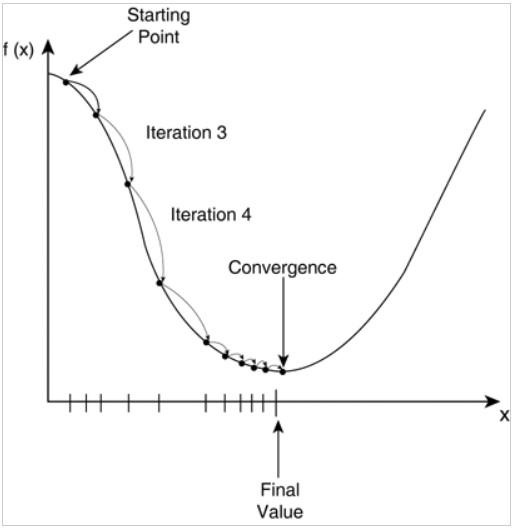
\includegraphics[width=0.5\textwidth]{2/figures/gradiente_descendiente.jpg}
					\caption{Ilustración del algoritmo gradiente descendiente. Fuente: \cite{tec_sancho2017descentgrad}}
					\label{2:fig14}
				\end{center}
			\end{figure}
			
			El Descenso del Gradiente, como también se le conoce, es el algoritmo de entrenamiento más simple y también el más extendido y conocido. Solo hace uso del vector gradiente, y por ello se dice que es un método de primer orden \parencite{tec_sancho2017descentgrad}. Un gradiente es la generalización de la derivada. Matemática, la derivada de una función mide la rapidez con la que cambia el valor de esta, según varié el valor de su variable independiente. La gradiente se calcula con derivadas parciales, por lo que al actualizar los coeficientes W para un tiempo t, se usa la regla \parencite{gl_iartificial2019descentgrad}.
			
			Donde alfa es el “ratio de aprendizaje”, el cual controla el tamaño de la actualización, si este es demasiado grande será más difícil encontrar los coeficientes que minimicen la función de coste o error; la actualización de W es proporcional al gradiente; y se usa la resta para ir en dirección opuesta al gradiente como en la Figura \ref{2:fig15}.
			\begin{figure}[h]
				\begin{center}
					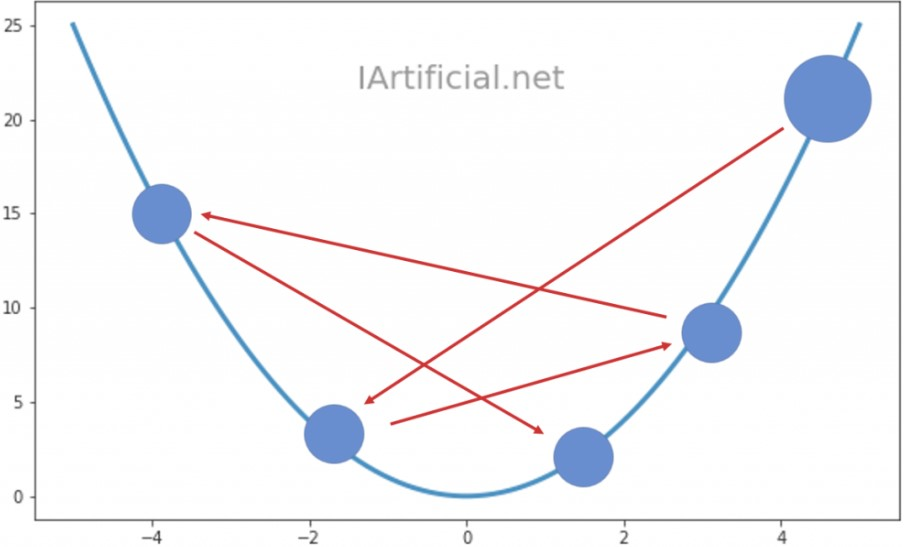
\includegraphics[width=0.5\textwidth]{2/figures/pesos_graddescen.jpg}
					\caption{Actualización de pesos W con el algoritmo. Fuente: \cite{gl_iartificial2019descentgrad}}
					\label{2:fig15}
				\end{center}
			\end{figure}
			
			\item \textbf{Propagación hacia atrás}: También conocido en inglés como \textit{Backpropagation}, es un método que consta de dos fases: en la primera se aplica un patrón, el cual se propaga por las distintas capas que componen la red hasta producir la salida de la misma. Luego, esta se compara con la salida deseada y se calcula el error cometido por cada neurona de salida. Estos errores se transmiten hacia atrás, partiendo de la capa de salida, hacia todas las neuronas de las capas intermedias [Fritsch, 1996] \parencite{tec_bertona2005algevol}. La actualización iterativa de los pesos que el algoritmo propone es mediante la siguiente fórmula:
			\begin{figure}[h]
				\begin{center}
					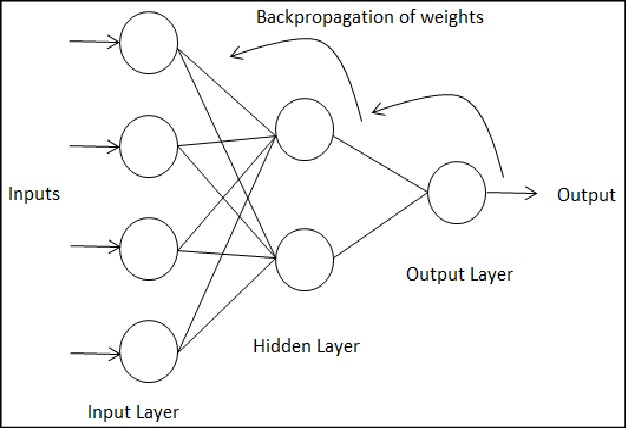
\includegraphics[width=0.5\textwidth]{2/figures/backpropagation.jpg}
					\caption{Capa oculta simple MLP con propagación hacia atrás. Fuente: \cite{gl_iartificial2019descentgrad}}
					\label{2:fig16}
				\end{center}
			\end{figure}
			
			Para entender mejor la teoría y la fórmula de actualización de pesos, se seguirá el siguiente ejemplo del conjunto de redes de la Figura \ref{2:fig17}.
			\begin{figure}[h]
				\begin{center}
					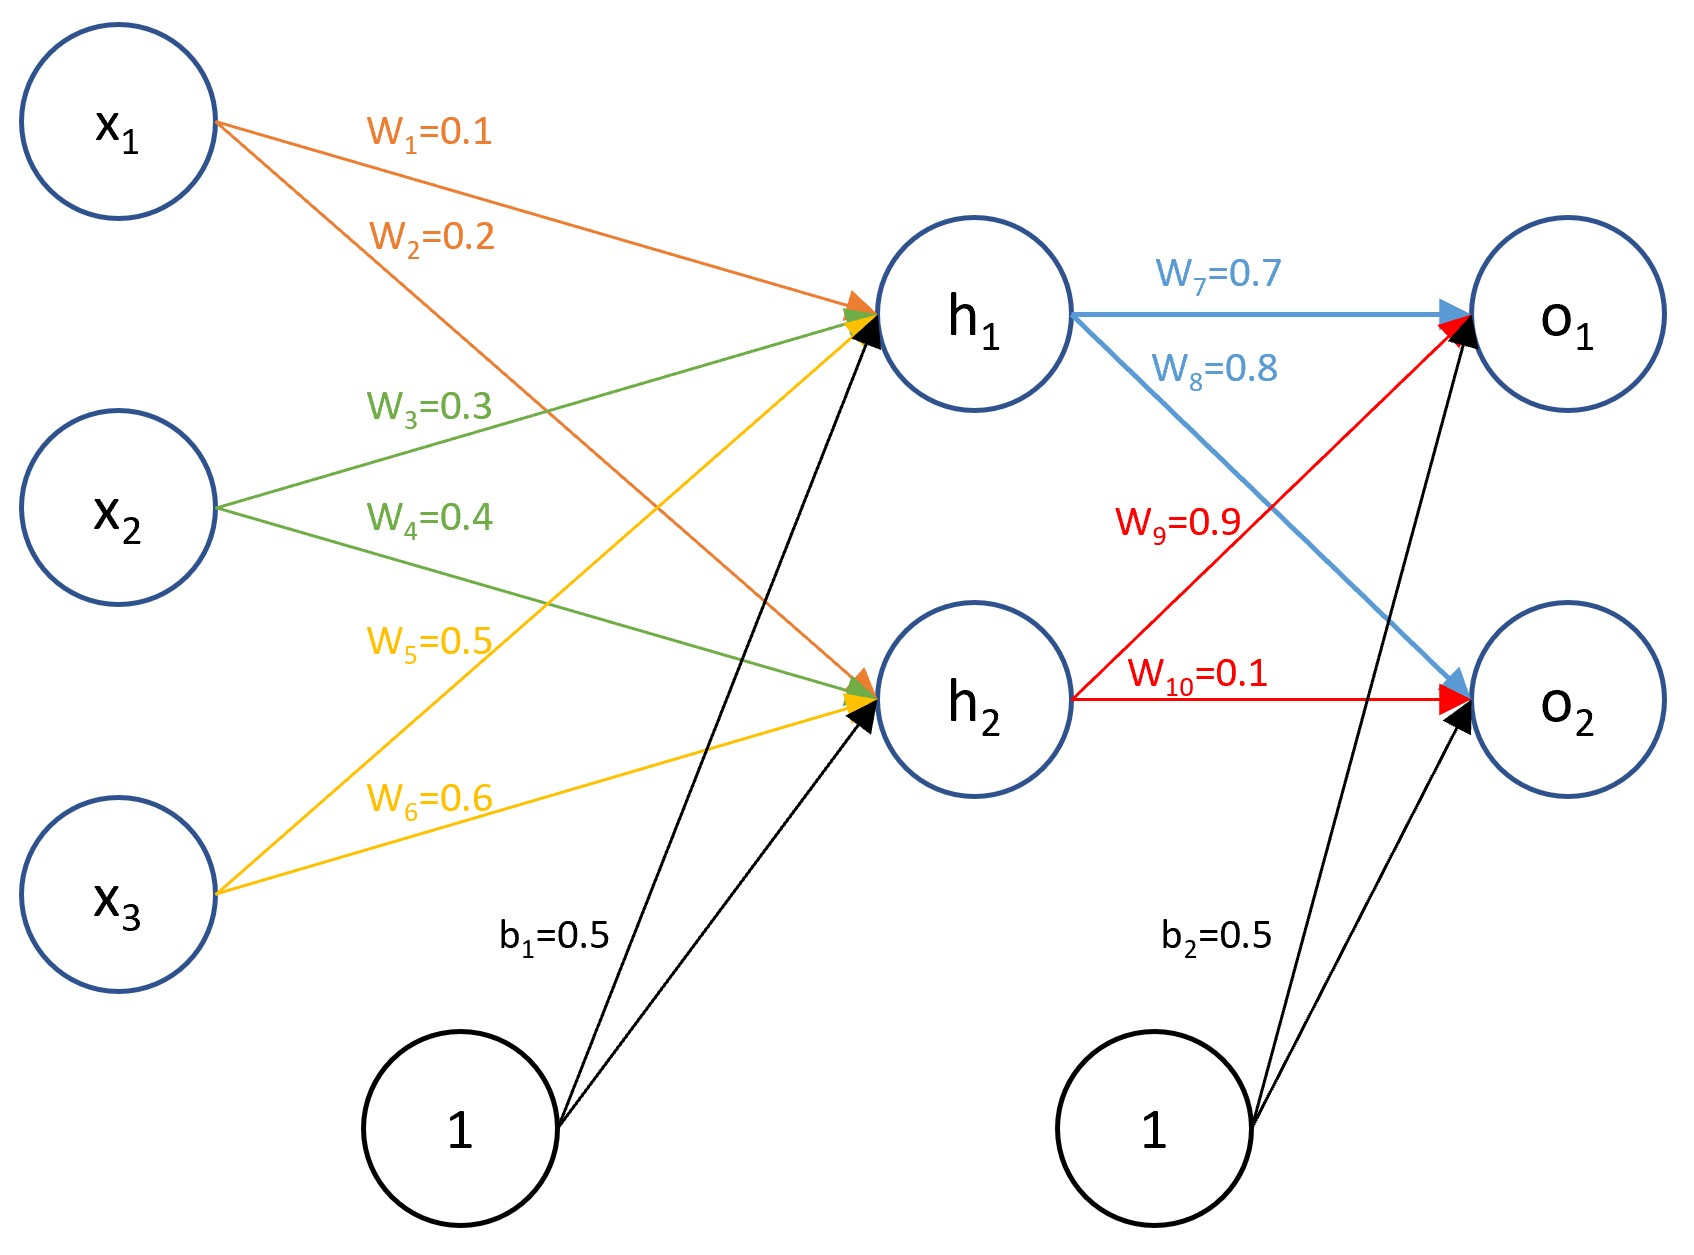
\includegraphics[width=0.5\textwidth]{2/figures/rna_pesos.jpg}
					\caption{Redes neuronales de ejemplo. Fuente: \cite{gl_ansrw2019backpropagation}}
					\label{2:fig17}
				\end{center}
			\end{figure}
			
			Se tiene una red neuronal con tres nodos de entradas (x1=1, x2=4 y x3=5) con dos pesos respectivos cada una (W1=0.1 y W2=0.2 para x1; W3=0.3 y W4=0.4 para x2; W5=0.5 y W6=0.6 para x3), dos capas ocultas (h1 y h2) con dos peso cada una (W7=0.7 y W8=0.8 para h1; W9=0.9 y W10=0.1 para h2) y dos nodos de salida (o1 y o2). El proceso normal para calcular el valor del nodo final se da, tanto con los nodos de entrada y los de capa oculta, mediante la sumatoria de producto de cada peso con su valor, es decir, mediante la fórmula de las RNA (colocar formula), al mismo tiempo que devuelve un valor del error cometido. Este último se calcula mediante la siguiente ecuación:
			Donde Tk es la salida correcta de cada nodo de salida, y Ok es la salida actual que cada uno genera. Con estos errores calculados, se retrocede hacia la capa oculta y se procede a calcular los nuevos pesos para sus nodos. La fórmula del cálculo de los mismos es:
			
			Donde Wjk representa el peso para cada nodo de la capa oculta, es decir, W7, W8, W9 y W10, los mismos que serán actualizados, L es el porcentaje de aprendizaje y Oj son los valores de estos dos nodos que entrarán a las salidas. Estos nuevos pesos permitirán redefinir los errores de ambos nodos, con una pequeña diferencia en su cálculo:
			
			El error de cada nodo de la capa oculta se obtiene multiplicando su valor por su complemento por la sumatoria del producto de sus pesos y los errores de los nodos de salida. Por ejemplo, para h1 sería (colocar fórmula).
			
			Finalmente, se retrocede hacia los nodos de entrada y se repite el mismo proceso para la actualización de sus pesos y errores.
		\end{itemize}
	\item \textbf{Función tangente hiperbólica}: Esta función está relacionada con una sigmoide bipolar. Sin embargo, sus salidas estarán en el rango de -1 y +1. Para redes neuronales, donde la velocidad es más importante que la forma de la función misma, es recomendable usar esta. Se representa como en la Figura \ref{2:fig18} y su fórmula para calcular su nuevo valor es:
	\begin{figure}[h]
		\begin{center}
			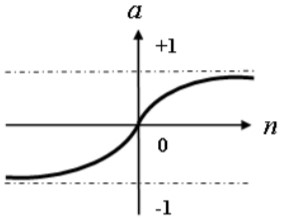
\includegraphics[width=0.3\textwidth]{2/figures/hiperbolica.jpg}
			\caption{Función de activación tangente hiperbólica. Fuente: \cite{pr_dorofki2012ann}}
			\label{2:fig18}
		\end{center}
	\end{figure}
	
	\item \textbf{Función puramente lineal (purelin)}: Esta función se caracteriza porque su salida es igual a su entrada debido a su linealidad. Normalmente se usa para obtener los mismos valores de la entrada. Se representa como en la Figura \ref{2:fig19} y su fórmula para calcular su nuevo valor es:
	\begin{figure}[h]
		\begin{center}
			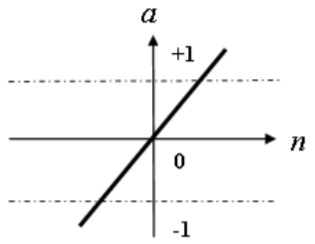
\includegraphics[width=0.3\textwidth]{2/figures/purelin.jpg}
			\caption{Función de activación puramente lineal. Fuente: \cite{pr_dorofki2012ann}}
			\label{2:fig19}
		\end{center}
	\end{figure}
	
	\item \textbf{Función Unidad Lineal Rectificada (ReLU)}: Esta función se caracteriza por, además de conservar los valores positivos, convertir los valores negativos de entrada en 0, esto con la finalidad de no considerarlos en la siguiente capa de convolución como en el caso de procesamiento de imágenes \parencite{gl_bigdata2019bigdata}. Si bien tiene un buen desempeño en redes convolucionales y es muy usada para el procesamiento de imágenes, al no estar acotada pueden morirse demasiadas neuronas \parencite{gl_calvo2018activrna}. Se representa como en la Figura \ref{2:fig20} y su fórmula para calcular su nuevo valor es:
	\begin{figure}[h]
		\begin{center}
			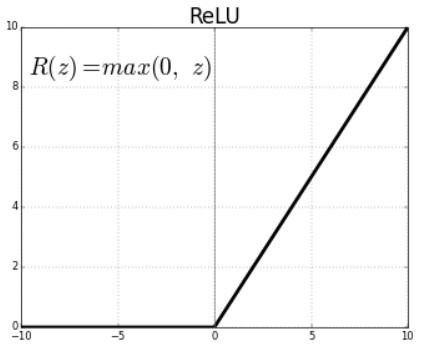
\includegraphics[width=0.3\textwidth]{2/figures/relu.jpg}
			\caption{Función de activación Unidad Lineal Rectificada. Fuente: \cite{gl_mlfa2019redesneuronales}}
			\label{2:fig20}
		\end{center}
	\end{figure}
	\end{itemize}
	
	Además de existir distintas funciones de activación, las redes neuronales artificiales se clasifican según la topología de red, siendo algunas de las más importantes \parencite{gl_calvo2017clasifrna}.
	
	\begin{itemize}
		\item \textbf{Red Neuronal Monocapa – Perceptrón simple}: Es la red neuronal más simple ya que está compuesta solamente de una capa de neuronas que componen varios nodos de entrada para proyectar una capa de neuronas de salida, como se aprecia en la Figura \ref{2:fig21}. Esta última capa se calcula usando la misma Ecuación 4 que implica la suma de productos de cada uno de los pesos de los nodos de entrada con sus instancias, añadiéndole finalmente el sesgo, aquel que controla la predisposición de la neurona a disparar un 1 o 0 independientemente de los pesos, para que el valor resultante se le aplique la función de activación que ayudarán a modelar funciones curvas o no triviales \parencite{gl_mlfa2019redesneuronales}.
		\begin{figure}[h]
			\begin{center}
				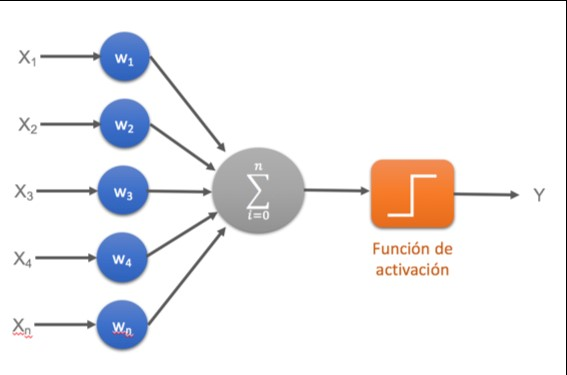
\includegraphics[width=0.65\textwidth]{2/figures/perceptron_simple.jpg}
				\caption{Ejemplo de perceptrón simple. Fuente: \cite{gl_calvo2017clasifrna}}
				\label{2:fig21}
			\end{center}
		\end{figure}
		
		\item \textbf{Red Neuronal Multicapa – Perceptrón multicapa}: Con arquitectura similar al perceptrón simple, con el añadido de contener capas intermedias entre la capa de neuronas de entrada y la de salida, conocidas como capas ocultas, como en el ejemplo de la Figura \ref{2:fig22}.
		\begin{figure}[h]
			\begin{center}
				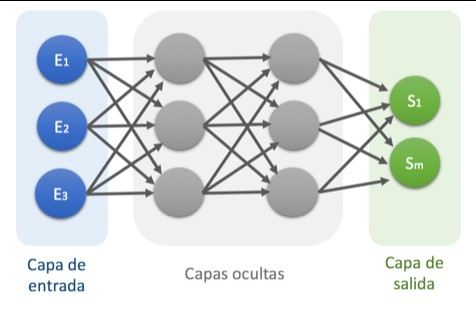
\includegraphics[width=0.65\textwidth]{2/figures/perceptron_multicapa.jpg}
				\caption{Ejemplo de perceptrón multicapa. Fuente: \cite{gl_calvo2017clasifrna}}
				\label{2:fig22}
			\end{center}
		\end{figure}
		
		\item \textbf{Redes Neuronales Convolucionales (CNN)}: También conocidas por su nombre en inglés \textit{Convolutional Neural Networks}, se diferencia del perceptrón multicapa en que cada neurona no necesita estar unida con todas las que le siguen, sino más bien solo con un subgrupo de estas con el fin de reducir la cantidad de neuronas necesarias para su funcionamiento, como se observa en la Figura \ref{2:fig23} \parencite{gl_calvo2017clasifrna}.
		\begin{figure}[h]
			\begin{center}
				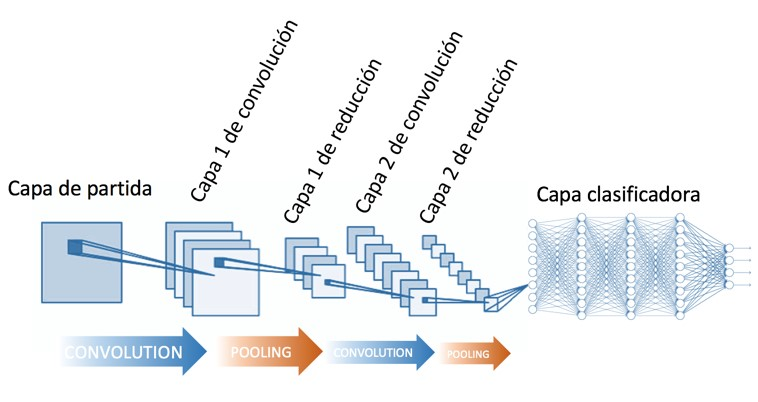
\includegraphics[width=0.65\textwidth]{2/figures/cnn.jpg}
				\caption{Ejemplo de red neuronal convolucional. Fuente: \cite{gl_calvo2017clasifrna}}
				\label{2:fig23}
			\end{center}
		\end{figure}
		
		Hoy en día, las redes neuronales convolucionales tienen múltiples usos desde que la idea fue concebida. Algunos de los problemas en las que pueden ser usados son de clasificación de objetos, recuperación de imágenes, detección y segmentación de objetos, distorsión y filtros de imágenes, por citar los ejemplos más comunes. El modelo de CNN más conocido es “AlexNet” (2012) por ser uno de los pioneros en clasificar imágenes \parencite{tec_li2019cnn}.
		
		Estas redes tienen su origen en el Neocognitron introducido por Fukushima en 1980 como modelo de red neuronal para el mecanismo de reconocimiento de patrón visual sin la enseñanza de un “profesor” (ver Figura \ref{2:fig24}), mismo que en el año 1998 sería mejorado por LeCun, Bottou, Bengio y Haffner al agregar un método de aprendizaje de gradiente aplicado al reconocimiento de documento basado en la propagación hacia atrás (ver Figura \ref{2:fig25}) \parencite{tec_li2019cnn}.
		\begin{figure}[htbp]
			\begin{center}
				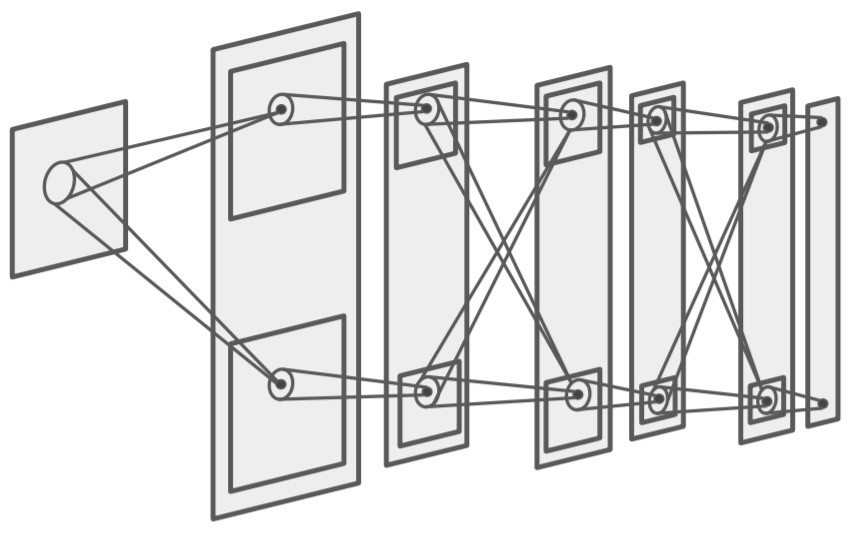
\includegraphics[width=0.6\textwidth]{2/figures/neocognitron.jpg}
				\caption{Modelo Neocognitron de Fukushima (1980). Fuente: \cite{tec_li2019cnn}}
				\label{2:fig24}
				
				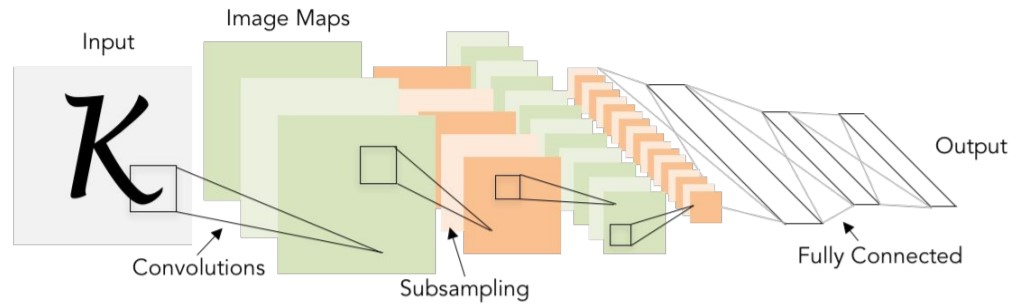
\includegraphics[width=0.8\textwidth]{2/figures/lenet5.jpg}
				\caption{Modelo LeNet-5 de LeCun (1998). Fuente: \cite{tec_li2019cnn}}
				\label{2:fig25}
			\end{center}
		\end{figure}
		
		Estos modelos se inspiraron en el estudio de la información visual en la corteza donde se ubican hasta 5 áreas. La primera, V1, contiene la información visual donde sus neuronas se ocupan de características visuales de bajo nivel, alimentando así a otras áreas adyacentes. Cada una de ellas se encarga de aspectos más específicos y detallados de la información obtenida. La idea de su implementación es la de solucionar el problema que surgen al escalar imágenes de mucha definición por las redes neuronales ordinarias. Por ello, este tipo de redes trabajan modelando de forma consecutiva piezas pequeñas de información para luego combinarlas en sus capas más profundas \parencite{tec_lopez2016cnnTF}.
		
		Su nombre deriva del concepto convolución. La convolución es un término en las matemáticas usado como operador matemático que convierte dos funciones f y g en una tercera función en donde la primera se superpone a una versión invertida y trasladada de la segunda, así como para denotar la distribución de la función de probabilidad de la suma de dos variables independientes aleatorias. Esta se da por la siguiente fórmula \parencite{tec_figueroa_convolucion}.
		
		Donde el rango puede variar entre un conjunto finito (como en la fórmula desde 0 hasta un valor t) o uno infinito.
		
		La estructura de las Redes Neuronales Convolucionales se constituye en tres tipos de capas \parencite{tec_lopez2016cnnTF}.
		\begin{itemize}
			\item \textbf{Capa convolucional (\textit{Convolutional Layer})}: Es la capa que hace distinta a esta red de otros tipos de redes neuronales artificiales. Se aplica la operación de la convolución, que recibe como entrada (\textit{input} en inglés) a la imagen para luego aplicarle un filtro (\textit{kernel} en inglés), devolviendo un mapa de las características de la imagen original, logrando así reducir el tamaño de los parámetros, como se observa en la Figura \ref{2:fig26}.
			\begin{figure}[h]
				\begin{center}
					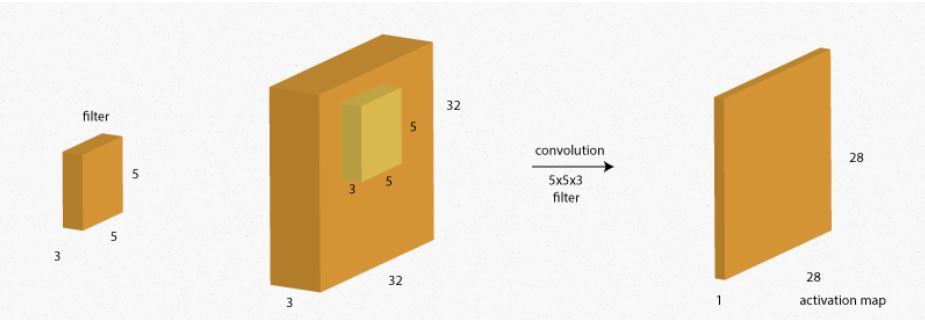
\includegraphics[width=0.8\textwidth]{2/figures/convolucion.jpg}
					\caption{Ejecución de la convolución en una entrada. Fuente: \cite{tec_lopez2016cnnTF}}
					\label{2:fig26}
				\end{center}
			\end{figure}
			
			Por ejemplo, en la anterior figura se tiene una imagen de entrada con dimensiones de 32 de alto, 32 de ancho y 3 de profundidad (32x32x3). A ella se le aplica un filtro de dimensiones (5x5x3) que recorrerá toda la imagen para extraer características de cada pixel. Tanto la profundidad de la entrada como del filtro siempre son iguales. El resultado de tomar un producto escalar entre el filtro y un pequeño fragmento de 5x5x3 de la imagen es un número, generando así un mapa de activación de nuevas dimensiones (28x28x1). Por cada n filtros aplicados a la entrada se generan n de estos mapas. Al final, la cantidad de mapas de activación determinará una nueva imagen de n de profundidad, como en la Figura \ref{2:fig27}.
			\begin{figure}[h]
				\begin{center}
					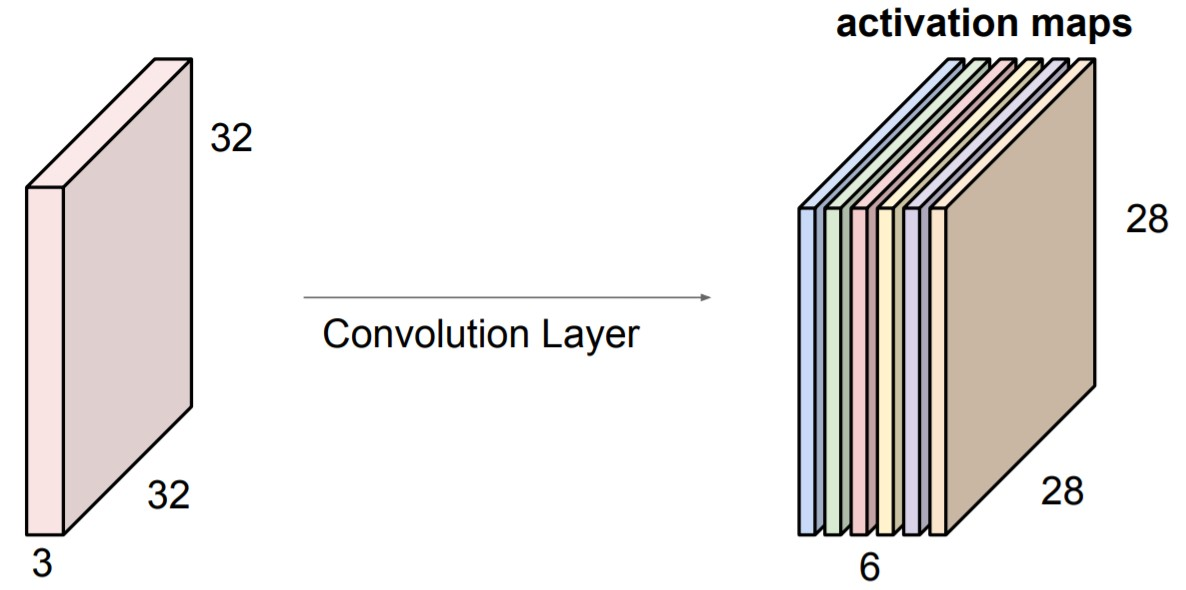
\includegraphics[width=0.7\textwidth]{2/figures/filtros_cnn.jpg}
					\caption{Generación de una nueva imagen a partir de filtros. Fuente: \cite{tec_li2019cnn}}
					\label{2:fig27}
				\end{center}
			\end{figure}
			
			Asimismo, cada vez que se aplica una convolución a una imagen, se aplicará una función de activación como en la secuencia de la Figura \ref{2:fig28}.
			\begin{figure}[h]
				\begin{center}
					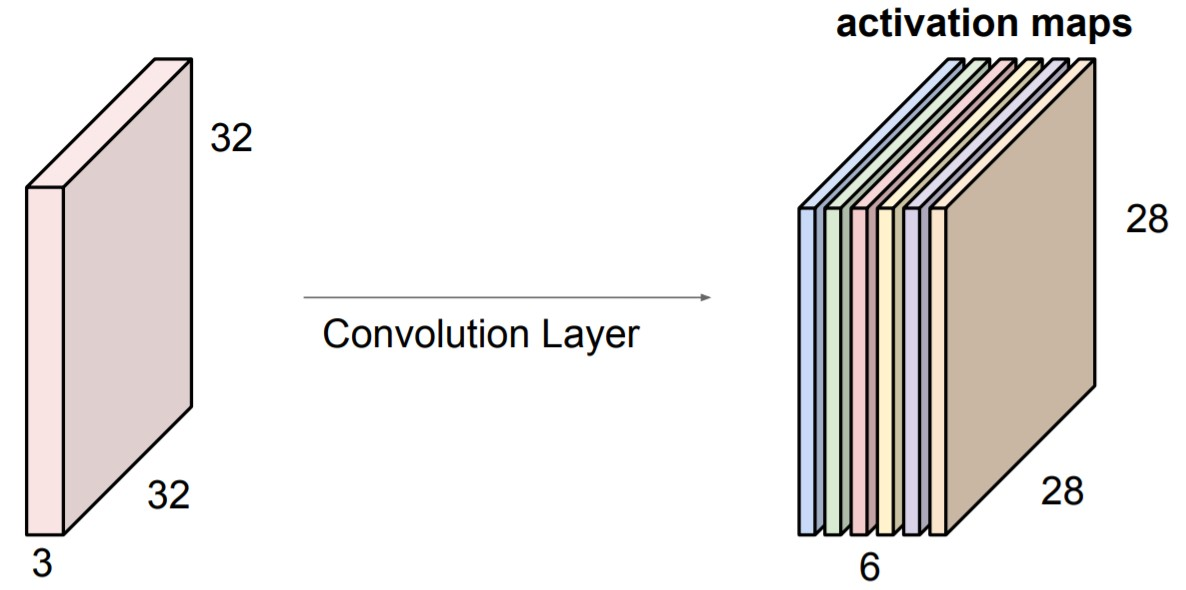
\includegraphics[width=0.7\textwidth]{2/figures/filtros_cnn.jpg}
					\caption{Secuencia de varias capas convolucionales. Fuente: \cite{tec_li2019cnn}}
					\label{2:fig28}
				\end{center}
			\end{figure}
			
			A nivel visual, en la Figura \ref{2:fig29} se aprecia un ejemplo de los resultados de aplicar varias convoluciones a una imagen.
			\begin{figure}[h]
				\begin{center}
					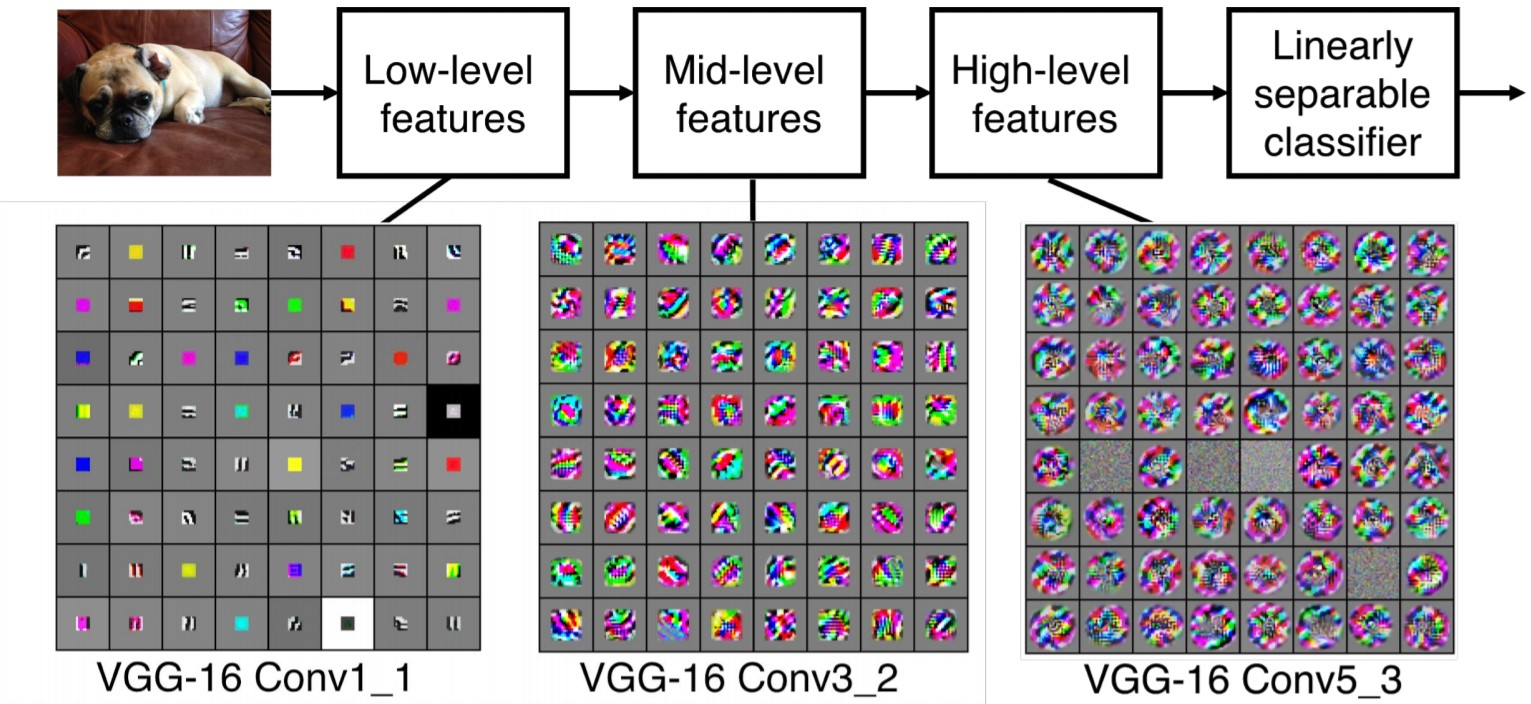
\includegraphics[width=0.75\textwidth]{2/figures/features_cnn.jpg}
					\caption{Extracción de características a partir de convoluciones. Fuente: \cite{tec_li2019cnn}}
					\label{2:fig29}
				\end{center}
			\end{figure}
			
			Finalmente, se calcula el volumen de la dimensión de la salida de la Figura \ref{2:fig30} mediante la siguiente ecuación:
			Se tiene una entrada de dimensiones (h x w x d).
			Se tiene un filtro de dimensiones (fh  x fw  x d).
			\begin{figure}[h]
				\begin{center}
					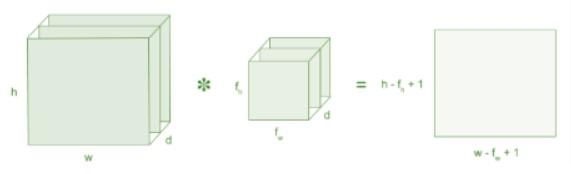
\includegraphics[width=0.75\textwidth]{2/figures/matriz_cnn.jpg}
					\caption{Ejemplo de matriz de imagen de entrada y un filtro. Fuente: \cite{tec_prabhu2018cnn}}
					\label{2:fig30}
				\end{center}
			\end{figure}
			
			\item \textbf{Capa de reducción (\textit{Pooling Layer})}: Esta capa le sucede a la capa convolucional (luego de aplicar la función de activación). Sirve principalmente para reducir las dimensiones espaciales del volumen de la entrada (alto x ancho) para la siguiente capa convolucional. Sin embargo, no afecta la profundidad de la misma. Esta operación que realiza se le conoce también como “reducción de muestreo” debido a que, si bien logra reducir las dimensiones para procesar mejor en la siguiente capa, también conlleva perder información. Por el contrario de lo que se piensa, además de reducir la sobrecarga del cálculo para las siguientes capas, el modelo se beneficia también disminuyendo el sobreajuste.
			
			Para determinar las dimensiones de la nueva imagen generada (siempre que sea cuadrada, es decir, lados iguales como en la Figura \ref{2:fig31}) con esta capa, se aplica la siguiente fórmula:
			
			Donde N es el tamaño del lado de la imagen de entrada, F es el tamaño del lado del filtro y Paso (Stride en inglés) es el número de desplazamiento de píxeles sobre la matriz de entrada. Por ejemplo, cuando el paso es 1, los filtros se mueven a 1 pixel por vez, cuando el paso es 2, se mueven a 2 píxeles (como en la Figura \ref{2:fig32}) y así sucesivamente (poner ref).
			\begin{figure}[htbp]
				\begin{center}
					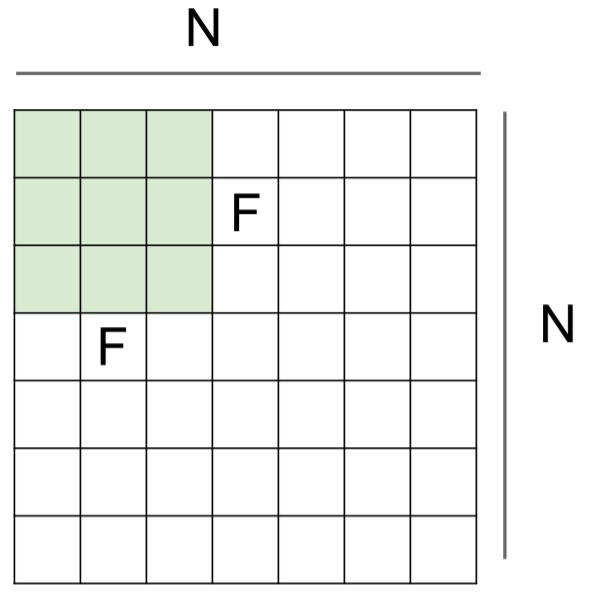
\includegraphics[width=0.3\textwidth]{2/figures/input_filter_cnn.jpg}
					\caption{Dimensiones de una entrada y un filtro. Fuente: \cite{tec_li2019cnn}}
					\label{2:fig31}
					
					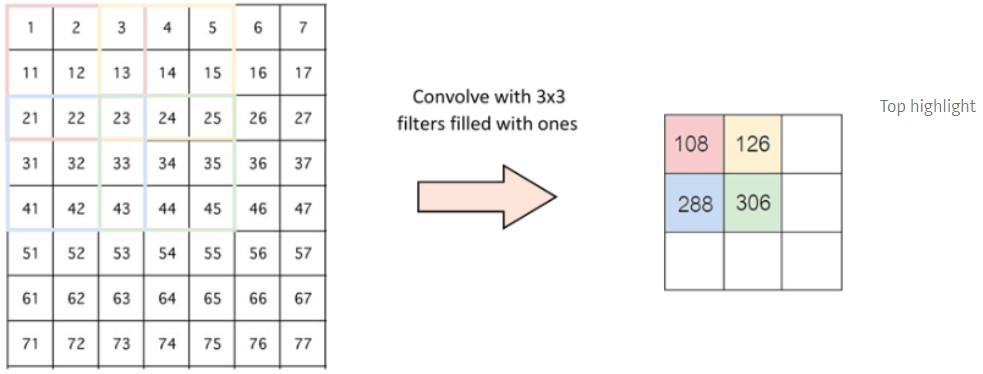
\includegraphics[width=0.7\textwidth]{2/figures/stride_cnn.jpg}
					\caption{Paso de 2 píxeles por parte de un filtro. Fuente: \cite{tec_prabhu2018cnn}}
					\label{2:fig32}
				\end{center}
			\end{figure}
			
			Si, por el contrario, se desea aplicar convolución a una imagen sin afectar sus dimensiones luego de pasar por la capa de reducción, se construye bordes de ceros de n píxeles. A este tamaño de borde se le llama Relleno (\textit{pad} en inglés), por lo que el tamaño de la nueva salida se obtiene mediante la siguiente fórmula:
			
			Existen diferentes tipos de reducción \parencite{tec_prabhu2018cnn}:
			\begin{itemize}
				\item Max Pooling: Toma el elemento más grande dentro del mapa de características.
				\item Average Pooling: Toma el promedio de los elementos dentro del mapa de características.
				\item Sum Pooling: Toma la suma total de los elementos dentro del mapa de características.
			\end{itemize}
			
			\item \textbf{Capa totalmente conectada (\textit{Fully Connected Layer})}: Al final de las capas de convolución y reducción, se usan redes completamente conectadas a cada pixel considerando que cada uno como una neurona separada al igual que en una red neuronal regular \parencite{tec_lopez2016cnnTF}. En esta capa, se aplana la matriz de todas las características obtenidas anteriormente a un vector y se alinea en una capa completamente conectada a una red neuronal (Figura \ref{2:fig33}).
			\begin{figure}[h]
				\begin{center}
					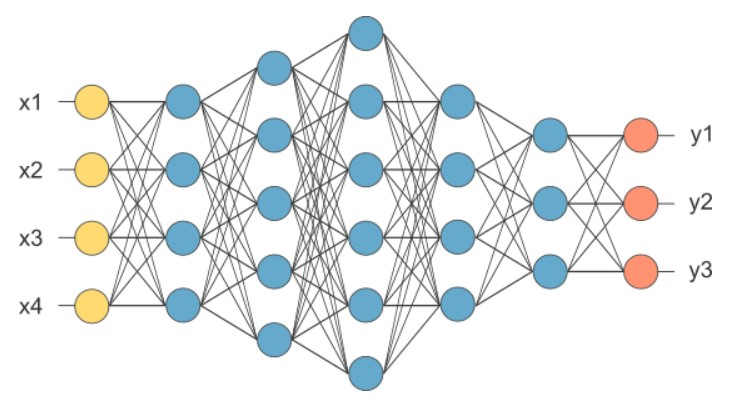
\includegraphics[width=0.75\textwidth]{2/figures/fully_conected_cnn.jpg}
					\caption{Aplanado de matrices luego de agrupar la capa. Fuente: \cite{tec_prabhu2018cnn}}
					\label{2:fig33}
				\end{center}
			\end{figure}
		\end{itemize}
		Para concluir, se muestra a continuación (Figura \ref{2:fig34}) la representación de la arquitectura completa de una Red Neuronal Convolucional resumiendo los conceptos anteriores.
		\begin{figure}[h]
			\begin{center}
				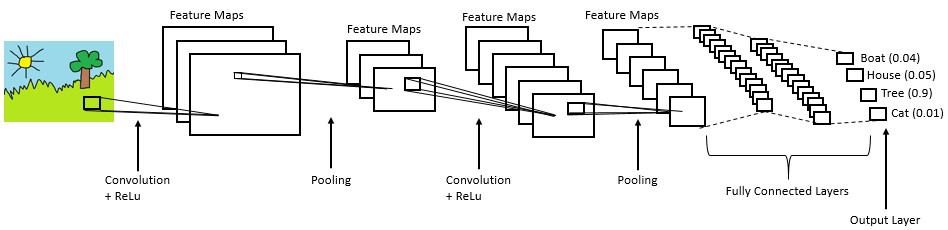
\includegraphics[width=0.8\textwidth]{2/figures/arquitectura_cnn.jpg}
				\caption{Arquitectura completa de una CNN. Fuente: \cite{tec_prabhu2018cnn}}
				\label{2:fig34}
			\end{center}
		\end{figure}
		
		\item \textbf{Redes Neuronales Recurrentes (RNN)}: También conocidas por su nombre en inglés \textit{Recurrent Neural Networks}, se caracterizan por no tener una estructura de capas como se aprecia en la Figura \ref{2:fig35}, sino más bien por permitir conexiones entre sus neuronas de manera arbitraria para crear temporalidad y que toda la red obtenga memoria. Todo esto permite generar una red muy potente para el análisis de secuencias, entre algunos ejemplos se mencionan el análisis de textos, sonidos o video \parencite{gl_calvo2018rnn}.
		\begin{figure}[h]
			\begin{center}
				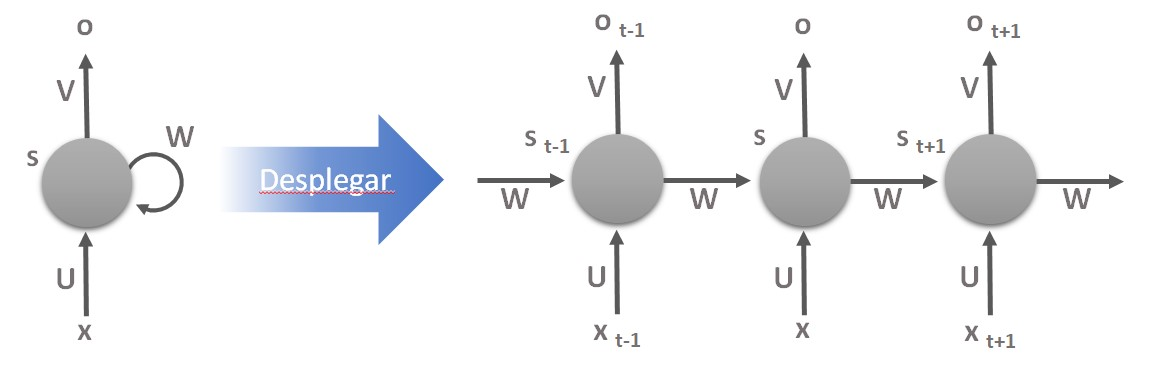
\includegraphics[width=0.8\textwidth]{2/figures/rnn_ejemplo.jpg}
				\caption{Ejemplo de red neuronal recurrente. Fuente: \cite{gl_calvo2018rnn}}
				\label{2:fig35}
			\end{center}
		\end{figure}
	\end{itemize}
	\item \textbf{Máquina de Vectores de Soporte (SVM)}: Es un algoritmo usado para tareas de regresión y clasificación, buscando un hiperplano en un espacio N-dimensional que clasifique claramente los puntos de datos a partir de la distancia máxima entre los puntos de datos de ambas clases. Para ello, maximiza la distancia del margen proporcionando cierto refuerzo para que los puntos de datos futuros puedan clasificarse con más confianza, es decir, que permita distinguir claramente dos clases, como se muestra en la Figura 39 (poner ref).
	
	Este algoritmo tiene sus orígenes en la década de los años 60 en Rusia, desarrollados por Vapnik y Chervonenkis. Inicialmente se enfocó en el reconocimiento óptico de caracteres (OCR). Más tarde, los clasificadores de Vectores de Soporte se volvieron competitivos con los mejores sistemas disponibles en ese momento para resolver no solamente el anterior tipo de problema, sino también abarcar tareas de reconocimiento de objetos. En 1998, se publicó el primer manual de estos algoritmos por Burges. Y debido a sus grandes resultados obtenidos en la industria, actualmente se usa con frecuencia en el campo del aprendizaje automático (poner ref).
	
	Los vectores de soporte hacen referencia a un pequeño subconjunto de las observaciones de entrenamiento que se utilizan como soporte para la ubicación óptima de la superficie de decisión (poner ref).
	
	Una Máquina de Vectores de Soporte aprende la superficie decisión de dos clases distintas de los puntos de entrada. Como un clasificador de una sola clase, la descripción dada por los datos de los vectores de soporte es capaz de formar una frontera de decisión alrededor del dominio de los datos de aprendizaje con muy poco o ningún conocimiento de los datos fuera de esta frontera. Los datos son mapeados por medio de un kernel Gaussiano u otro tipo de kernel a un espacio de características en un espacio dimensional más alto, donde se busca la separación máxima entre clases. Cuando es traída de regreso al espacio de entrada, la función de frontera puede separar los datos en todas las clases distintas, cada una formando un agrupamiento. Esta teoría se basa en la idea de minimización de riesgo estructural (SRM), demostrando en muchas aplicaciones tener mejor desempeño que otros algoritmos de aprendizaje tradicional como las redes neuronales para resolver problemas de clasificación (poner ref).
	
	Cabe mencionar que hay casos en que el conjunto de datos de dos clases puede ser separables no necesariamente de forma lineal. En las Figura 40 y Figura 41 se observan casos linealmente y no linealmente separables, respectivamente.
	
	Lo que se debe hacer para el primer caso es crear el hiperplano a través de una función lineal w*z+b=0 y, definido el par (w,b), separar el punto xi según la función:
	
	Para el segundo caso, debido a su mayor complejidad, se puede introducir algunas variables no-negativas a la función del hiperplano para hallar su valor óptimo; o también es viable utilizar una función kernel que calcule el producto punto de los puntos de entrada en el espacio de características Z, como se aprecia en la Figura 42.
	
	\item \textbf{Árboles de Decisión}: Representación visual de decisiones y toma de decisiones utilizada en la minería de datos para derivar una estrategia y alcanzar un objetivo particular. Se dibuja boca abajo con su raíz en la parte superior. Consta de nodos internos, los cuales se subdividen en ramas o bordes y su contenido, las hojas o decisiones (poner ref).
	
	Un árbol de decisión toma como entrada un objeto descrito a través de un conjunto de atributos y devuelve una “decisión”. Estos pueden ser discretos o continuos. La salida puede tomar cualquiera de estos dos tipos de valores; en el caso que aprenda una función tomando valores discretos se le denominará clasificación, y en el caso que la función sea continua será llamada regresión. En las clasificaciones booleanas, es decir de dos valores o binaria, clasificará como verdadero (positivo) o falso (negativo). Para alcanzar una decisión, el árbol desarrolla una serie de pruebas a través de sus nodos y las ramas que salen del nodo son etiquetadas con los valores posibles de dicha propiedad. Además, cada nodo hojas del árbol representa el valor que ha de ser devuelto si es alcanzado (poner ref).
	
	Por ejemplo, representando un ejemplo de este algoritmo, se ilustra en la Figura 43 para decidir si se debe esperar por una mesa en un restaurante.
\end{itemize}

\subsection{Natural Language Processing (NLP)}

 